\documentclass{article}
\usepackage[utf8]{inputenc}
 \usepackage{enumerate}
 \usepackage[T1]{fontenc}
\usepackage{cite}
%\usepackage{caption}
%\usepackage{subcaption}
\usepackage{mathtools}
\usepackage{stackengine}
\def\delequal{\mathrel{\ensurestackMath{\stackon[1pt]{=}{\scriptstyle\Delta}}}}
\usepackage{amsmath,amssymb,amsfonts}
\usepackage{amsmath,epsfig,cite,amsfonts,amssymb,psfrag,subfigure}
\usepackage{graphicx}
\usepackage{blindtext}
\usepackage{textcomp}
\usepackage{xcolor}
\usepackage{algorithm}
\usepackage[noend]{algpseudocode}
\usepackage{amsthm}
\def\BibTeX{{\rm B\kern-.05em{\sc i\kern-.025em b}\kern-.08em
    T\kern-.1667em\lower.7ex\hbox{E}\kern-.125emX}}
\allowdisplaybreaks
\newtheorem{remark}{Remark}
\newtheorem{theorem}{Theorem}
\newtheorem{lemma}{Lemma}
\newtheorem{proposition}{Proposition}
\newtheorem{corollary}{Corollary}
\newcommand{\diag}{\mathop{\mathrm{diag}}}
\DeclareMathOperator{\E}{\mathbb{E}}
\usepackage[margin=0.7in]{geometry}
\usepackage[export]{adjustbox}

\title{Reporte de inventario de eviencias}
\author{Natalia Galeano Valerio}
\date{Octubre 2019}

\begin{document}


\baselineskip 12pt

\vspace*{30mm}

\begin{center}

\textbf{\Large Research Plan} \\
\vspace{10mm}
\textbf{Department of Electrical and Computer Engineering}\\
\vspace{20mm}
%{\large University of Oulu}\\
{\large University of Tehran}\\
\vspace{20mm}
\end{center}
\vspace{10mm}
{\scriptsize Provisional title:}\\
Dynamic Resource Allocation in O-RAN Architecture using Network Slicing\\

\vspace{20mm}

{\scriptsize Candidate name}\\
Mojdeh Karbalaee Motalleb \\
\vspace{3mm}



{\scriptsize Supervisor name:}\\
Dr. Onel Lopez\\
\vspace{3mm}


\pagebreak
\section{Introduction}
Open radio access network (O-RAN), as the integration and expansion of cloud RAN (C-RAN) and xRAN, or C-RAN and virtual RAN (vRAN), is expected to be a key technology in 5G networks to enhance the RAN performance extensively. 

O-RAN, as illustrated in Fig. \ref{fig:c11}, separates RAN into three different units, namely Radio Unit (O-RU), Distributed Unit (O-DU), and Central Unit (O-CU).
The architecture of O-RAN contains other principal logical nodes called Orchestration and Automation,
RAN Intelligent Controller (RIC)- Near Real-Time and O-Cloud. 
One of the necessities of the new generation of wireless networks is its intelligence.
Based on the requirement of an intelligent wireless network, O-RAN offers machine learning techniques such as deep learning and reinforcement learning. The two logical nodes RIC-Non Real-Time (which is placed in Orchestration and Automation node) and RIC- Near Real-Time, implement the algorithms for network intelligence
\cite{niknam2020intelligent,ORANArch,ORANML}.
\begin{figure*}
  \centering 
    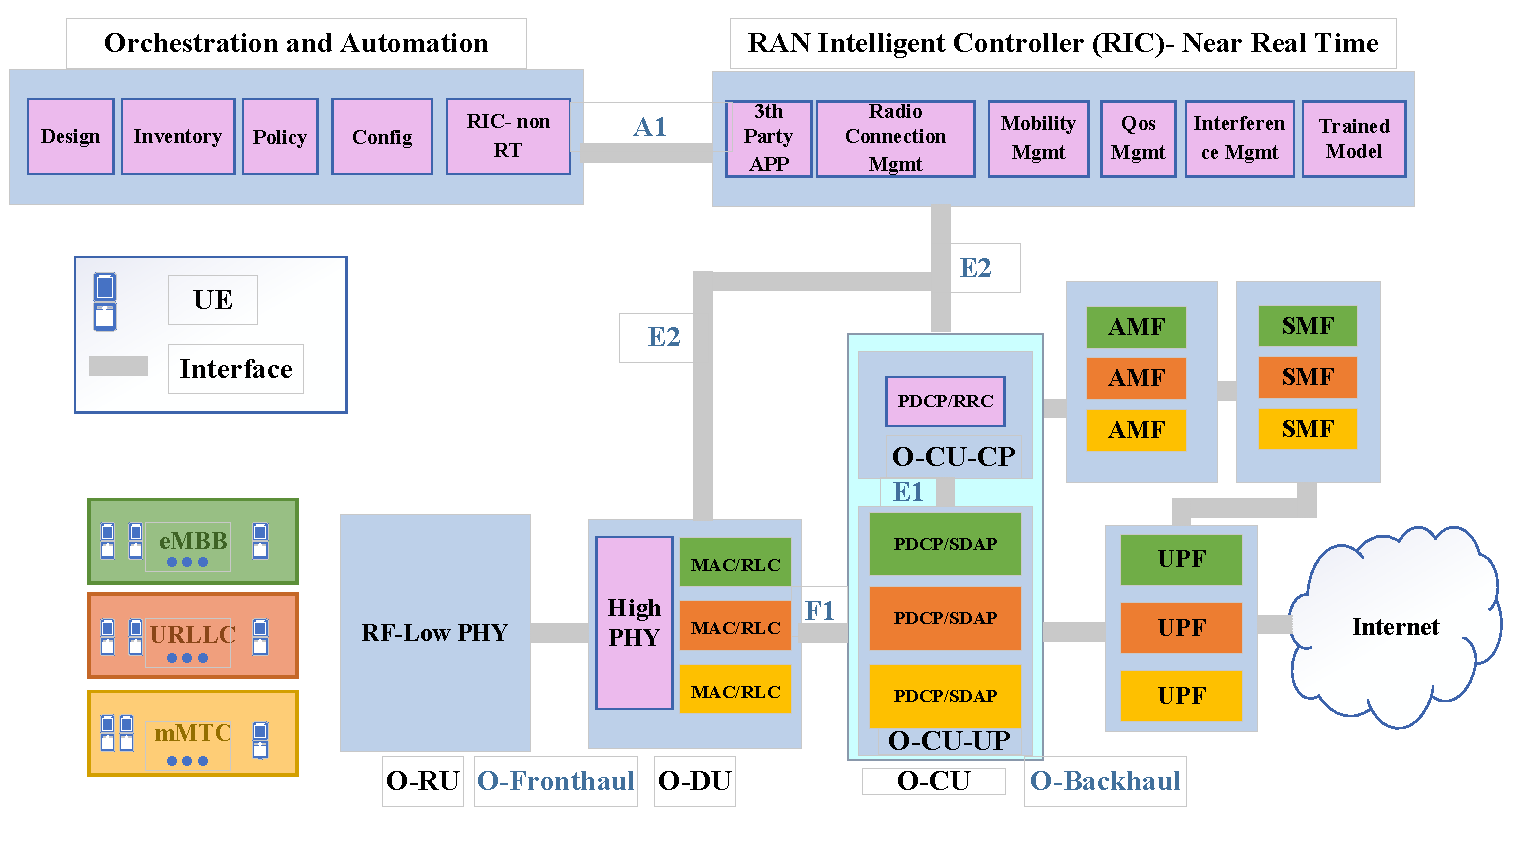
\includegraphics[scale = 0.5]{finalDraw.pdf}
    %\includegraphics[max height=30cm,max width=9.5cm]{Drawing15.eps}
    %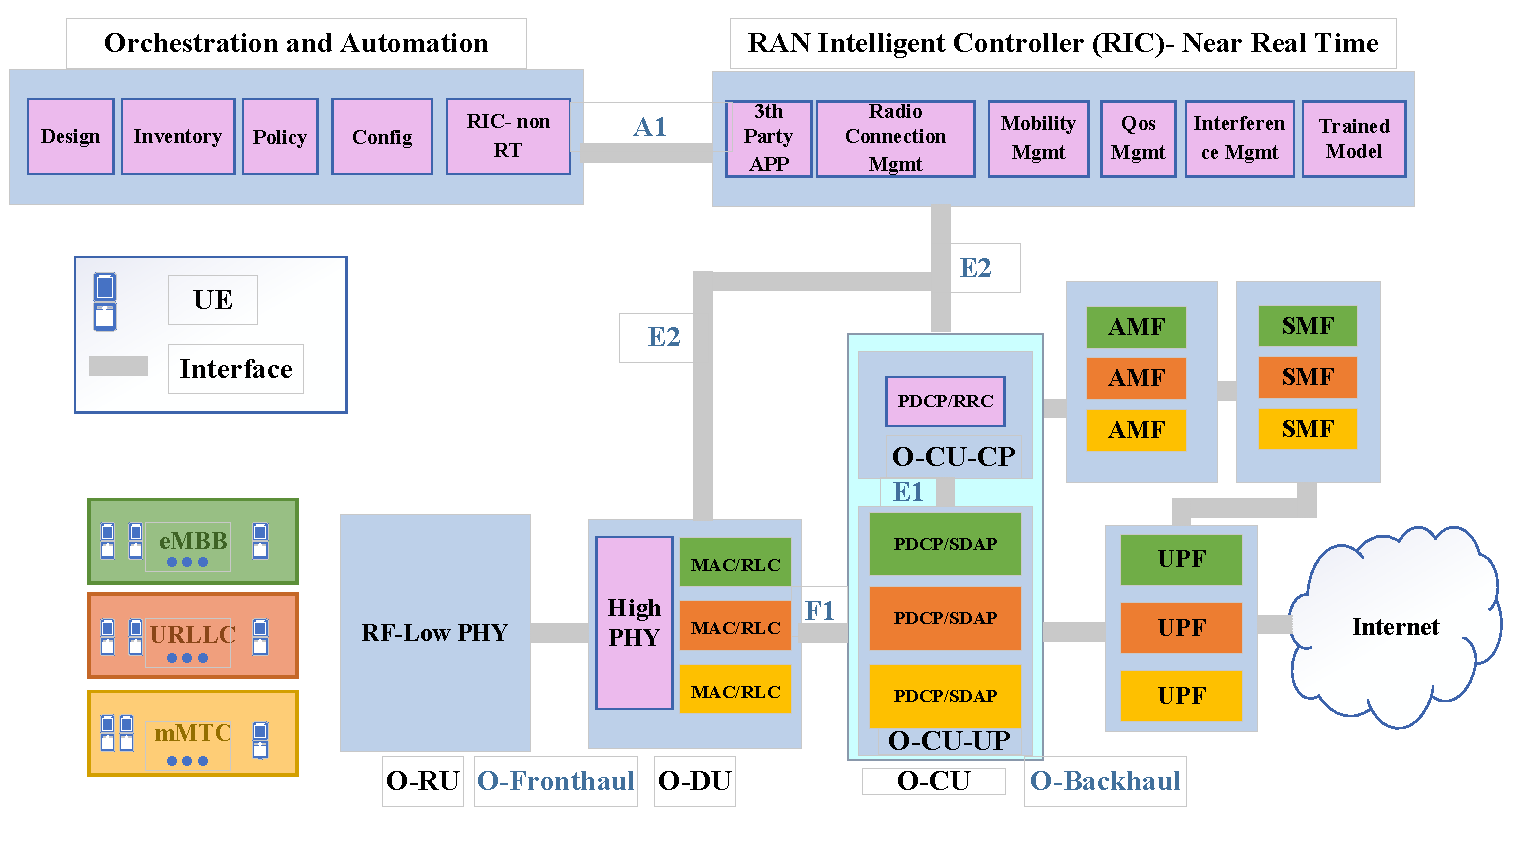
\includegraphics[width=\textwidth]{finalDraw.pdf}
  \caption{Network sliced ORAN system}
  \label{fig:c11}
\end{figure*}


One of the goals of the next generation of mobile systems is to strictly meet the stringent QoS demands of the different services introduced in 5G , i.e., eMBB, URLLC, and mMTC. Network slicing is a promising solution to obtain the QoS for each type of service. 

In addition, according to the high complexity of RAN slicing and incapability of the traditional model-based methods, dynamic machine learning becomes the best solution for these problems.
 Generally, there are two kinds of deep reinforcement learning methods for solving dynamic problems. The first class is value-based such as Deep-Q-Network, and the second class is policy-based problems such as
deep deterministic policy gradient (DDPG). The first class can only solve the discrete action space problems, which are integer programming. The second class can solve by searching the optimal policy, which is the actor-critic method \cite{alsenwi2021intelligent,yan2019intelligent,mei2021intelligent}.
\section{Machine Learning Methods}
In this project, we want to solve the problem of dynamic resource allocation in the O-RAN system using RAN slicing. Here, we assume that we have three service types served by three slices, namely, eMBB, URLLC, and mMTC. Each service requires its specific QoS.
Our system model has a two time-scale. In the first time-scale, we want to solve the problem of obtaining the optimal number of VNFs and the assignment of PRBs for each slice. In the second time-scale, we seek to solve the power allocation and PRB assignment of each UEs in each slice. We use deep reinforcement learning since we want to solve the dynamic resource allocation.

\subsection{Requirement of Deep Reinforcement Learning}
A few pioneers developed an intelligent RAN slicing architecture incorporating DL (deep learning) technologies into network slicing and achieving automatic RAN slicing control due to the complexity of RAN slicing and the untenability of conventional models-based approaches. 
Since 5G networks are complex, and the wireless environment is dynamic and unpredictable, Reinforcement Learning (RL) is ideal for optimizing dynamic decision-making in real-time.

To extract the system's inherent value, DL uses model-free methodology features and makes decisions based on historical data sets. 
By interacting with an unknown environment, Deep Reinforcement Learning (DRL) performs self-optimization of system performance, which has received considerable attention from research.
Therefore, DRL approaches, which combine deep neural networks (DNNs) with reinforcement learning, are particularly promising because they can cope with large state and action spaces.
DRL methods have already been used for resource allocation in 5G networks.

In this project, we would like to allocate resources using DRL. This project has a two time-scale. The large time-scale considers the optimal number of VNFs and the assignment of a PRB to each slice, which is the action of our problem.







\newpage
To measure the effectiveness of each state or state action pair, DQN constructs a value function model. Through optimizing the value function model, DQN derives the appropriate control policy implicitly. Although DQN has good sample efficiency and stable performance, it has the disadvantage that its action space must be a discrete variable set. 

Because we have many states and actions and the action is discrete, we use deep Q learning and want to compare it with double deep Q learning to solve the first part of our problem. The Q network is a multi-perceptron network and also we would like to compare it with a LSTM (long short term memory) to find the best Q network. 

Actor-Critic is a Temporal Difference(TD) version of Policy gradient. It has two networks: Actor and Critic. The actor decided which action should be taken and critic inform the actor how good was the action and how it should adjust. The learning of the actor is based on policy gradient approach. In comparison, critics evaluate the action produced by the actor by computing the value function. 
In the second-time scale, we use actor-critic method such as deep deterministic policy gradient (DDPG) since we have a continuous actions and states.
The DDPG method can be used to solve continuous stochastic optimization problems, which are more common in network resource management. Also, Proximal Policy Optimization(PPO) and softmax policy gradient are two another methods that we want to compare it for our problem. 
\subsection{Software Requirement}
In this part, we discuss software requirements and the implementation of the algorithms mentioned above. 
We can implement the DRL methods using python and Matlab 2021. In this project, we choose python programming to write our codes. In python, we have different libraries to implement deep learning methods such as PyTorch, TensorFlow, and Keras. Here, we use PyTorch 1.10.1 (required cuda 10.2) for writting the deep Q networks. PyTorch can only be used in Ubuntu systems and we required an Ubuntu 20.04 Os for our project. 
Moreover, for this project a GPU GeForce RTX 2080 ti can be a perfect solution for processing of our codes. 
The RTX2080 has tensor-core which will be used in games that support DSLL feature. Tensor-core is a feature strongly advertised with Nvidia Volta GPU that is meant for professional usage such as deep learning and machine learning.
The Tensor cores in each RTX GPU are capable of performing extremely fast deep learning neural network processing.

Moreover, we want to compare our simulations with optimal solution which is a brute-force algorithm and takes lots of time in each loop and we need high RAM (32G) and SSD hard disk (256G) to compare it with the optimal solution.  
\bibliographystyle{IEEEtran} 
\bibliography{ref}
%\begin{thebibliography}{9}
%\bibitem{Hunt}
%Sally Hunt, ``Making Competition Work in Electricity,'' John Wiley , pp.23-30, Fev, 2002.



%\end{thebibliography}
\vspace{20mm}


\end{document}
